\subsection{Sentence Salience}

\begin{frame}{Sentence Salience}

    \begin{itemize}
        \item Lots of recent work on deep nets for sentence extractive news 
            summarization. 
            \begin{itemize}
                \item Cheng and Lapata, (2016); Nallapati et al., (2016); Narayan et al., (2018), and more...
            \end{itemize}~\\
        \item \alert{Salience} is modeled as a \alert{sentence classification} problem, 
            \begin{itemize}
        \item i.e. salience =
            probability of including a sentence in an extract summary.
    \end{itemize}~\\

        \item Multiple architecture tweaks in each work
            \begin{itemize}
                \item Difficult to tell
            what is actually driving improvements.
    \end{itemize}
    \end{itemize}

\end{frame}
\begin{frame}{Summarizer Architecture}
  \begin{center}
      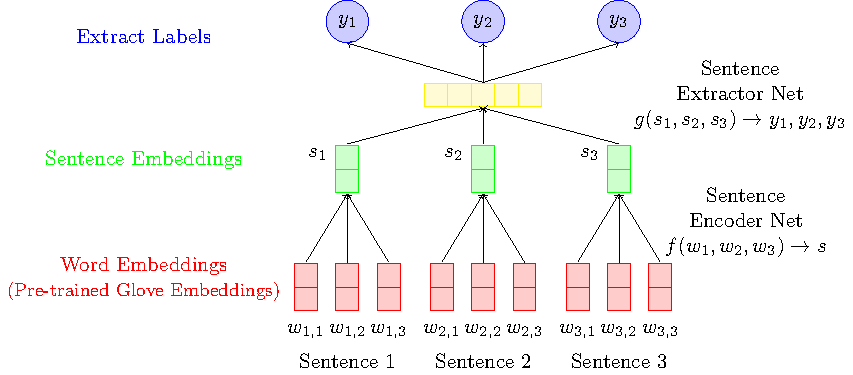
\includegraphics[scale=.85]{3_deep_learning_models_of_salience/image_texs/arch/arch.pdf}
%    \begin{tikzpicture}
%      \node at (0.4,-.75) {Sentence 1};
%      \node at (4.9,-.75) {Sentence 2};
%      \node at (8.9,-.75) {Sentence 3};
%      \node (w1) at (0,0) 
%      {\large $\textsc{Enc}\left(w^{(1)}_1,
%         w^{(1)}_2, w^{(1)}_3 \right)$};
%
%      \node (w2) at (4.5,0) 
%      {\large $\textsc{Enc}\left(w^{(2)}_1, 
%         w^{(2)}_2, w^{(2)}_3  \right)$};
%      \node (w3) at (8.6,0) 
%      {\large $\textsc{Enc}\left(w^{(3)}_1, 
%         w^{(3)}_2 \right)$};
%
%      \node (s1) at (3,2) {\large $s_1$};
%      \node (s2) at (4,2) {\large $s_2$};
%      \node (s3) at (5,2) {\large $s_3$};
%      
%        \draw[->,thick] (w1.north) -- (s1.south); 
%        \draw[->,thick] (w2.north) -- (s2.south);
%        \draw[->,thick] (w3.north) -- (s3.south);
%        \node (ext) at (3.6,2) {\large $\textsc{Ext}\Big( 
%        \quad\quad\quad\;\;\;\;\;\;\;\;\;\;\; \Big)$};
%        \node (y1) at (3,3.5) {\large $y_1$};
%        \node (y2) at (4,3.5) {\large $y_2$};
%        \node (y3) at (5,3.5) {\large $y_3$};
%        \draw[->,thick] (s1.north) -- (y1.south);
%        \draw[->,thick] (s2.north) -- (y2.south);
%        \draw[->,thick] (s3.north) -- (y3.south);
%
%    \end{tikzpicture}
  \end{center}
\end{frame}


\begin{frame}{Sentence Salience}

    \begin{itemize}
            \uncover<1->{
        \item We experiment with several popular sentence encoder methods.
            \begin{itemize}
                \item Word Embedding Averaging 
                \item Recurrent Neural Nets (RNNs)
                \item Convolutional Neural Nets (CNNs)
            \end{itemize}~\\
        }
        \uncover<2->{
        \item We experiment with two state of art sentence extractor
            architectures (Nallapati et al., 2016) and (Cheng \& Lapata, 2016),
    and ~\\~\\}
    \uncover<3>{
        \item propose simplified versions of each (RNN and Seq2Seq, respectively).

        }
    \end{itemize}

\end{frame}


%\begin{frame}{Sentence Encoders}
% \begin{columns}[t]
%  \column{.32\textwidth}
%   \centering
%   Averaging Encoder\\~\\
%   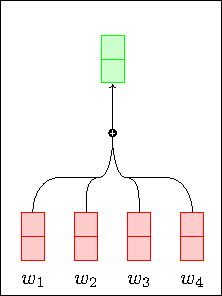
\includegraphics[]{images/section3/avg_encoder.pdf}\\
%  \column{.32\textwidth}
%   \centering
%   RNN Encoder\\~\\
%   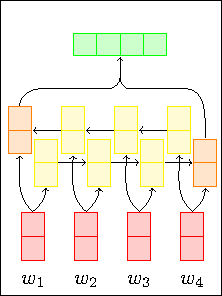
\includegraphics[]{images/section3/rnn_encoder.pdf}\\
%  \column{.32\textwidth}
%   \centering
%   CNN Encoder\\~\\
%   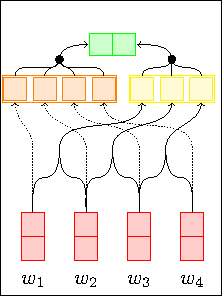
\includegraphics[]{images/section3/cnn_encoder.pdf}\\
% \end{columns}
%
%~\\
%We use pretrained (Wikipedia/Gigaword) Glove word embeddings.
%
%\end{frame}



\begin{frame}{Sentence Extractors}
 \begin{columns}[t]
  \column{.4\textwidth}
   \centering
   SummaRunner Extractor\\
   (Nallapati et al. 2016)\\
   \only<1>{
   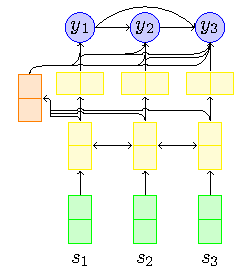
\includegraphics[scale=.65]{3_deep_learning_models_of_salience/image_texs/sr1/sr1.pdf}\\}
   \only<2>{
   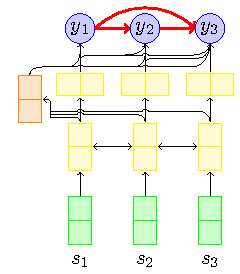
\includegraphics[scale=.65]{3_deep_learning_models_of_salience/image_texs/sr2/sr2.pdf}\\}
   RNN Extractor (ours)\\
   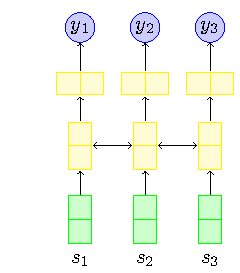
\includegraphics[scale=.65]{3_deep_learning_models_of_salience/image_texs/rnn/rnn.pdf}
  \column{.6\textwidth}
   \centering
   Cheng \& Lapata Extractor\\
   (Cheng and Lapata, 2016)\\
   \only<1>{
   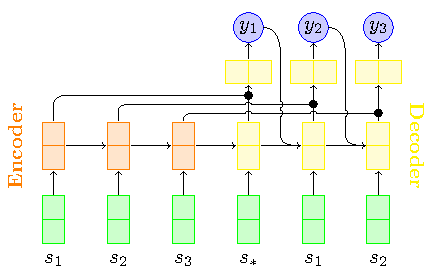
\includegraphics[scale=.65]{3_deep_learning_models_of_salience/image_texs/cl1/cl1.pdf}\\}
   \only<2>{
   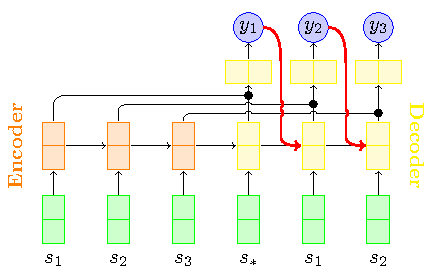
\includegraphics[scale=.65]{3_deep_learning_models_of_salience/image_texs/cl2/cl2.pdf}\\}
   Seq2Seq Extractor (ours)\\
   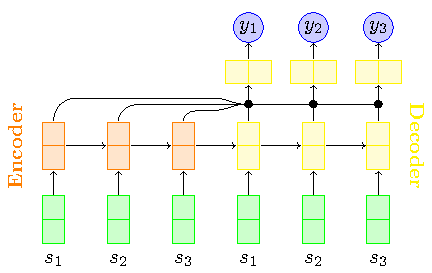
\includegraphics[scale=.65]{3_deep_learning_models_of_salience/image_texs/s2s/s2s.pdf}
 \end{columns}

\end{frame}

\begin{frame}{Datasets}
  \begin{center}
      \begin{tabular}{ gcgcgc }
%      \toprule
      \textbf{Dataset} & \textbf{Genre} & \textbf{Train} & \textbf{Valid} & \textbf{Test} &
        \textbf{Refs} \\
        \midrule
        CNN/DailyMail & News &  287,113 & 13,368 & 11,490 & 1\\
        \hline
        NYT & News & 44,382 & 5,523 & 6,495 & 1.93\\
        \hline
        \makecell{Reddit \\(Ouyang et al., 2017)} & \makecell{Personal\\Narratives} & 404 & 24 & 48 & 2 \\
        \hline
        PubMed & \makecell{Medical\\Journal\\Articles}& 21,250 & 1,250 & 2,500 & 1\\
      \bottomrule
    \end{tabular}
  \end{center}
  ~\\
%
  Sizes of the training, validation, test splits for each dataset
  and the average number of test set human reference summaries per document.



\end{frame}




\begin{frame}{Sentence Extractor Evaluation}
    \begin{center}
        Simpler extractors are just as good if not better! ~\\~\\

\begin{tabular}{cgc}
 &  \multicolumn{2}{c}{\textbf{Rouge-2 Recall}}\\
 \toprule
 \alert{\underline{\textbf{Sentence Extractor}}} & \textbf{CNN/DM} & \textbf{NYT} \\
 \midrule
% \textsc{Lead}    &  24.4  \\
% \hline
 \textsc{RNN}     & 25.4  & 34.7  \\
 \hline
 \textsc{Seq2Seq} & \alert{\textbf{25.6}} &\alert{\textbf{35.7}} \\
 \hline
 \textsc{Cheng \&  Lapata} & 25.3 & 35.6 \\
 \hline
 \textsc{SummaRunner}  & 25.4 & 35.4 \\
% \hline
%    \textsc{Oracle} &  36.2 \\
 \bottomrule
\end{tabular}
\end{center}
\end{frame}

\begin{frame}{Sentence Extractor Evaluation}
    \begin{center}

        Simpler extractors are just as good if not better! ~\\~\\
        Similar story on non-news datasets. ~\\~\\

\begin{tabular}{cgc}
 &  \multicolumn{2}{c}{\textbf{Rouge-2 Recall}}\\
 \toprule
 \alert{\underline{\textbf{Sentence Extractor}}} & \textbf{Reddit} & \textbf{PubMed} \\
 \midrule
% \textsc{Lead}    &  24.4  \\
% \hline
 \textsc{RNN}     & 11.4  & 17.0  \\
 \hline
 \textsc{Seq2Seq} & \alert{\textbf{13.6}} &\alert{\textbf{17.7}} \\
 \hline
 \textsc{Cheng \&  Lapata} & 13.6 & 17.7 \\
 \hline
 \textsc{SummaRunner}  & 13.4 & 17.2 \\
% \hline
%    \textsc{Oracle} &  36.2 \\
 \bottomrule
\end{tabular}
\end{center}

\uncover<2>{ ~\\~\\ Similar results for choice of sentence encoder: averaging is as good as RNN and CNN encoders.}




\end{frame}

\begin{frame}{Additional experiments}

What are these models learning? 

~\\

How are important sentences identified? Lexical information?

\begin{enumerate}
    \item<2-> Word Embedding Fine Tuning: 
        \begin{itemize}
            \item<3-> No significant improvement! 
            \item<3-> In fact, worse performance on average (.3-.7 pts worse on news) 
        \end{itemize}
                ~\\
    \item<4-> POS class ablations: Remove nouns, verbs, adj/adv, and function
        words.
        \begin{itemize}
            \item<5-> News datasets mostly unaffected (-0.1pt)
            \item<5-> Reddit sees modest drop (-2pts) when removing adj./adv.
        \end{itemize}
    ~\\
    \item<6-> Sentence order shuffling:
        \begin{itemize}
            \item<7-> Large drops in performance on news and PubMed. 
        \end{itemize}
        
\end{enumerate}



\end{frame}


\begin{frame}{Shuffled vs In-Order}

 \begin{center}
     \begin{tabular}{ccL{2cm}m{1cm}L{1cm}m{2cm}} 
   \toprule
   \textbf{Ext.} & \textbf{Order} & 
   \textbf{CNN/DM} & \textbf{NYT} & \textbf{Reddit} & \textbf{PubMed} \\
   \midrule
%?   \multirow{2}{*}{RNN} 
%?       & In-Order & 
%?       \textbf{25.4} & \textbf{34.7} & \textbf{22.7} \\
%?       & Shuffled & 
%?               22.8 &          25.0  &         18.2  \\
   \multirow{2}{*}{Seq2Seq}
       & In-Order & 
   \textbf{25.6} & \textbf{35.7} &  \textbf{13.6} & \textbf{17.7} \\ 
       & Shuffled & 
   21.7  &         25.6  &  \textbf{13.5}  &       14.9  \\
   \bottomrule
  \end{tabular}
 \end{center}

 ~\\

 Shuffled model is trained on shuffled sentence order documents.

 ~\\

 Both models evaluated on in-order data.


~\\ 
 Large \textbf{performance drops} on news and PubMed!

 \uncover<2>{
~\\
    \begin{itemize}
        \item Simple network architectures good enough. 
        \item Without care, document structure dominates learning. 
    \end{itemize}
 }

\end{frame}


